% !TEX TS-program = xelatex
% !TEX encoding = UTF-8 Unicode
% !Mode:: "TeX:UTF-8"

%This file contains the LaTeX code of my laboratory report for my ICS II course.
%Author: 张作柏/Zuobai Zhang <17300240035@fudan.edu.cn>

% This is a simple template for a LaTeX document using the "article" class.
% See "book", "report", "letter" for other types of document.

\documentclass[12pt]{article} % use larger type; default would be 10pt

\usepackage[utf8]{inputenc} % set input encoding (not needed with XeLaTeX)

%%% Examples of Article customizations
% These packages are optional, depending whether you want the features they provide.
% See the LaTeX Companion or other references for full information.

%%% PAGE DIMENSIONS
\usepackage[top=1.05in, bottom=0.95in, left=0.90in, right=1.10in]{geometry}
%\usepackage{geometry} % to change the page dimensions
\geometry{a4paper} % or letterpaper (US) or a5paper or....
% \geometry{margin=2in} % for example, change the margins to 2 inches all round
% \geometry{landscape} % set up the page for landscape
%   read geometry.pdf for detailed page layout information

\usepackage{graphicx} % support the \includegraphics command and options

% \usepackage[parfill]{parskip} % Activate to begin paragraphs with an empty line rather than an indent

%%% PACKAGES
\usepackage{booktabs} % for much better looking tables
\usepackage{array} % for better arrays (eg matrices) in maths
\usepackage{paralist} % very flexible & customisable lists (eg. enumerate/itemize, etc.)
\usepackage{verbatim} % adds environment for commenting out blocks of text & for better verbatim
\usepackage{subfig} % make it possible to include more than one captioned figure/table in a single float
% These packages are all incorporated in the memoir class to one degree or another...

%%% HEADERS & FOOTERS
\usepackage{fancyhdr} % This should be set AFTER setting up the page geometry
\pagestyle{fancy} % options: empty , plain , fancy
%\renewcommand{\headrulewidth}{0pt} % customise the layout...
\lhead{}\chead{}\rhead{}
\lfoot{}\cfoot{\thepage}\rfoot{}

%%% SECTION TITLE APPEARANCE
\usepackage{sectsty}
\allsectionsfont{\sffamily\mdseries\upshape} % (See the fntguide.pdf for font help)
% (This matches ConTeXt defaults)

%%% ToC (table of contents) APPEARANCE
\usepackage[nottoc,notlof,notlot]{tocbibind} % Put the bibliography in the ToC
\usepackage[titles,subfigure]{tocloft} % Alter the style of the Table of Contents
\renewcommand{\cftsecfont}{\rmfamily\mdseries\upshape}
\renewcommand{\cftsecpagefont}{\rmfamily\mdseries\upshape} % No bold!
\usepackage{titletoc}
\titlecontents{section}
              [1.5cm]
              {\bf \large}%
              {\contentslabel{1.8em}}%
              {}%
              {\titlerule*[0.5pc]{$\cdot$}\contentspage\hspace*{0.6cm}}%
		   [\vspace{0.5em}]
\titlecontents{subsection}
              [1.8cm]
              {\normalsize}%
              {\contentslabel{2.0em}}%
              {}%
              {\titlerule*[0.5pc]{$\cdot$}\contentspage\hspace*{0.6cm}}%
		   [\vspace{0.4em}]
\titlecontents{subsubsection}
              [2.1cm]
              {\small}%
              {\contentslabel{2.5em}}%
              {}%
              {\titlerule*[0.5pc]{$\cdot$}\contentspage\hspace*{0.6cm}}%
		   [\vspace{0.4em}]


\usepackage[UTF8]{ctex}
\usepackage{fancyhdr}
\usepackage{enumerate}
\usepackage{indentfirst}
\usepackage{extramarks}
\usepackage{titling}
\usepackage{listings}
\usepackage{xcolor}
\usepackage{fontspec}
\usepackage[CJKbookmarks=true,colorlinks,linkcolor=black]{hyperref}
\setmainfont{Times New Roman}



\definecolor{mygreen}{rgb}{0,0.6,0}  
\definecolor{mygray}{rgb}{0.9,0.9,0.9}  
\definecolor{mymauve}{rgb}{0.58,0,0.82}  
  
\lstset{ %  
  backgroundcolor=\color{mygray},   % choose the background color; you must add \usepackage{color} or \usepackage{xcolor}  
  basicstyle=
	{
		\footnotesize
		\fontspec{Consolas}
	},        % the size of the fonts that are used for the code  
  breakatwhitespace=false,         % sets if automatic breaks should only happen at whitespace  
  breaklines=true,                 % sets automatic line breaking  
  captionpos=bl,                    % sets the caption-position to bottom  
  commentstyle=
	{
		\color{mygray}
		\fontspec{Consolas Italic}
	},    % comment style  
  deletekeywords={...},            % if you want to delete keywords from the given language  
  escapeinside={\%*}{*)},          % if you want to add LaTeX within your code  
  extendedchars=true,              % lets you use non-ASCII characters; for 8-bits encodings only, does not work with UTF-8  
  %frame=shadow,                    % adds a frame around the code  
  keepspaces=true,                 % keeps spaces in text, useful for keeping indentation of code (possibly needs columns=flexible)  
  keywordstyle=
	{
		\color{blue}
		\fontspec{Consolas Bold}
	},       % keyword style  
  %language=Python,                 % the language of the code  
  morekeywords={*,...},            % if you want to add more keywords to the set  
  numbers=none,                    % where to put the line-numbers; possible values are (none, left, right)  
  numbersep=5pt,                   % how far the line-numbers are from the code  
  numberstyle=\tiny\color{mygray}, % the style that is used for the line-numbers  
  rulecolor=\color{black},         % if not set, the frame-color may be changed on line-breaks within not-black text (e.g. comments (green here))  
  showspaces=false,                % show spaces everywhere adding particular underscores; it overrides 'showstringspaces'  
  showstringspaces=false,          % underline spaces within strings only  
  showtabs=false,                  % show tabs within strings adding particular underscores  
  stepnumber=1,                    % the step between two line-numbers. If it's 1, each line will be numbered  
  stringstyle=\color{blue},     % string literal style  
  tabsize=4,                       % sets default tabsize to 2 spaces  
  %title=myPython.py                   % show the filename of files included with \lstinputlisting; also try caption instead of title  
}  


%%% END Article customizations

%%% The "real" document content comes below...

%\title{\textbf{Digital Logic and Computer Design Report}}
\title{\textbf{MIPS流水线处理器实验报告}}
\author{张作柏\\17300240035}
%\date{} % Activate to display a given date or no date (if empty),
         % otherwise the current date is printed 

\begin{document}
\begin{sloppypar}
\maketitle

\pagestyle{fancy}
\lhead{\textbf{{\thetitle}}}
\rhead{\textbf{\nouppercase{\firstleftmark}}}
\cfoot{\thepage}

\thispagestyle{empty}
\tableofcontents
\clearpage

\setcounter{page}{1}

\section{流水线处理器简介}

流水线技术是提高数字系统吞吐量的有效手段。通过将单周期处理器分解成5个流水线阶段来构成流水线处理器。因此,可以在流水线中同时执行5条指令,时钟频率几乎可以提高5倍。

流水线被划分为五个阶段,每个阶段完成一个操作:取指令(Fetch),译码(Decode),执行(Execute),存储器(Memory)和写回(Writeback)。
\begin{itemize}
\item {\bf 取指}: 处理器从指令存储器中读取指令。
\item {\bf 译码}: 处理器从寄存器文件中读取源操作数并对指令译码以便产生控制信号。
\item {\bf 执行}: 处理器使用ALU执行计算。
\item {\bf 存储器}: 处理器读或写数据存储器。
\item {\bf 写回}: 处理器将结果协会到寄存器文件。
\end{itemize}

\begin{figure}[h]
\centering
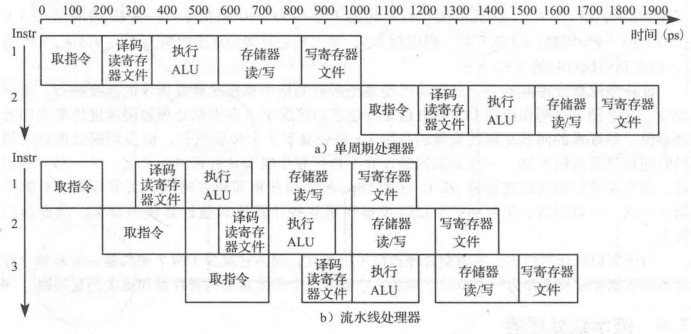
\includegraphics[width =0.95\linewidth]{figure/timestep.png}
\end{figure}

上图对比了单周期处理器与流水线处理器的时序图\footnote{图源于教材256页}。可以看出,流水线的吞吐量明显高于单周期,也说明了流水线处理器的高效性。。

流水线系统中的核心问题是冲突(Hazard),即当后一条指令需要前一条指令的计算结果,而前一条指令还没有执行完时就会发生冲突。在这里,我们可以使用重定向、阻塞和刷新三种处理方法。

\newpage
\section{部件分析}

多周期处理器中大部分器件都与单周期相似,在此只列出新添加或发生改动的部件,其余请参考我的单周期报告。

\subsection{触发器flopr}

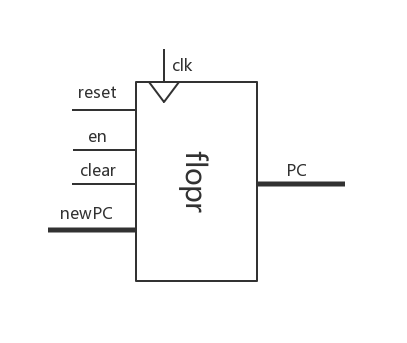
\includegraphics[width =0.35\linewidth]{figure/flopr.jpg}

流水线中,除了本来datapath中的寄存器,我们还需要添加两两阶段之间的状态寄存器。而为了支持状态的阻塞和刷新操作,我们需要给寄存器加入同步清零功能。所以,寄存器共有异步清零reset、使能en和同步清零clear三个控制口。

\subsection{比较器eqcmp}

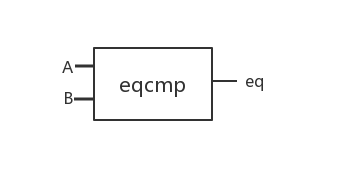
\includegraphics[width =0.3\linewidth]{figure/eqcmp.jpg}

为了提前预测beq和bne是否跳转,我们需要在decode阶段预判两个操作数是否相等,所以需要添加一个比较器。A与B都是32位数字,当A==B时,eq=1,当A!=B时,eq=0。


\subsection{数据通路Datapath}
\noindent
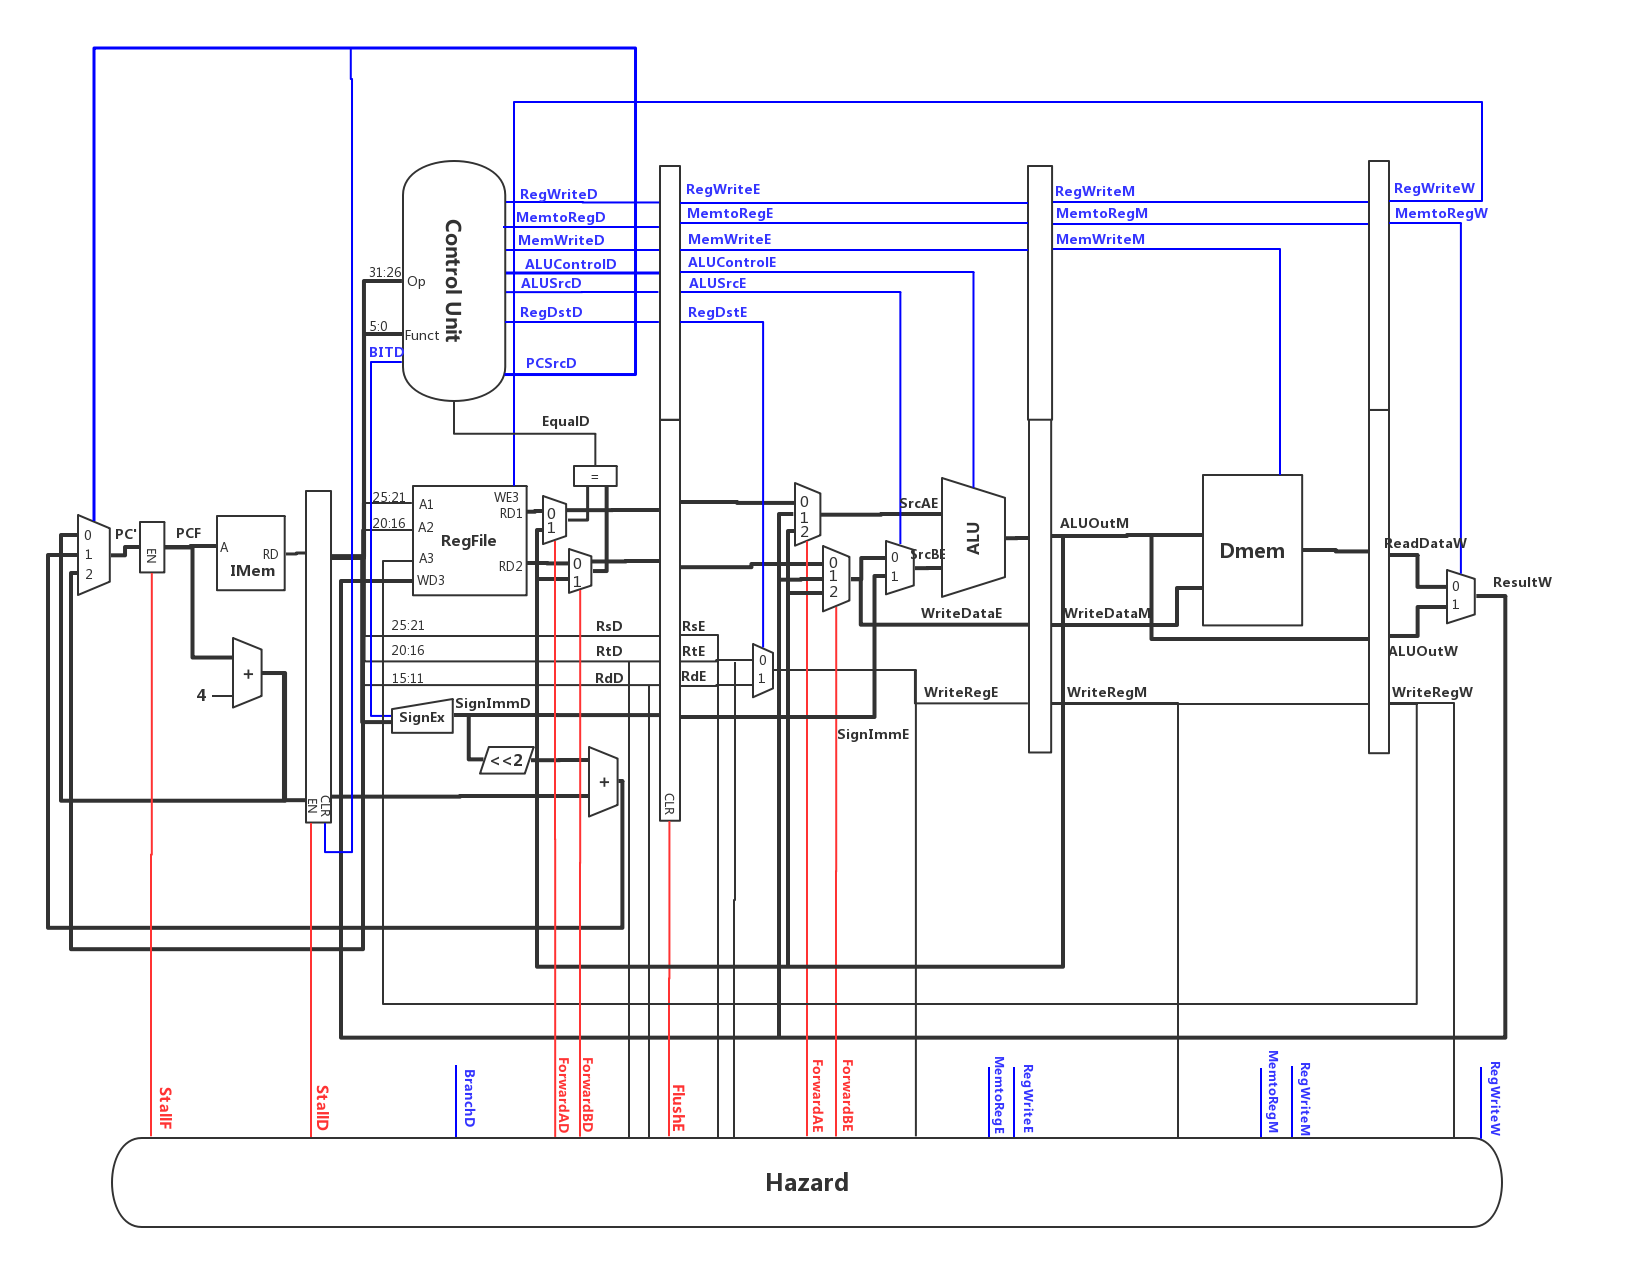
\includegraphics[width =\linewidth]{figure/Datapath.jpg}

{\bf 功能说明}:因为与单周期相比很多部件都没有改变,所以这里只说明变化的部分。
\begin{itemize}
\item 左侧PC寄存器,添加了PCEn信号,控制寄存器写入逻辑,只在需要更新PC值的状态才将PCEn设置为1。
\item 左侧二路选择器,因为Dmem与Imem合二为一了,所以要通过IorD信号选择读取指令还是读取数据。
\item 左侧Instr寄存器,只有当需要读指令时,才将IRWrite信号设为1,其余状态则需要存储原先的指令。
\item 中间A、B两个寄存器用于存从RegFile中读出来的值,因为这些值可能会延迟一个状态使用,所以需要用寄存器储存。
\item 中间SrcA是ALU的A参数,由ALUSrcA信号控制:当ALUSrcA为0时,选择PC值作为运算对象(常用作计算下一指令的PC值);当ALUSrcB为1时,选择A寄存器的值作为运算对象,用于R型和部分I型指令。
\item 中间SrcB是ALU的B参数,由ALUSrcB信号控制:当ALUSrcB为00时,选择B寄存器的值作为运算对象,用于R型指令;当ALUSrcB为01时,选择4作为运算对象,用于计算下一条指令的PC;当ALUSrcB为10时,选择移位前的立即数作为运算对象,用于I型指令;当ALUSrcB为11时,选择移位后的立即数作为运算对象,用于计算jal、bne、beq指令跳转的目标地址。
\item 右侧ALUOut寄存器用于存储ALU运算的结果,以供下一周期使用。
\item 右侧四路选择器用于选择PC的值,由PCSrc信号控制,共四种选择:ALUResult(下一指令PC),ALUOut(jal、bne、beq指令的跳转地址)、PCJump(j指令的跳转地址)、A(jr指令的跳转地址)。
\end{itemize}

\subsection{控制模块Controller}

\subsubsection{控制信号说明}

\subsubsection{实现细节}


最后,在每个时钟上升沿到来时,用nextstate更新state:
\begin{lstlisting}[language=Verilog]  
\end{lstlisting}  

\subsection{冲突处理模块Hazard}



\newpage
\section{冲突处理与额外指令分析}

\subsection{冲突处理}

图中未标出的控制变量均默认为0。

\subsection{额外指令分析}


\subsubsection{移位指令sll}

注意到,这里没有为移位指令单独设计状态,而是将其作为普通的R-Type指令来处理。因为我改造了ALU,把移位数传到了ALU中,这样就ALU就可以直接根据funct进行移位操作了。过程与其它R-Type指令完全一样,无需增加新的状态。

\subsubsection{函数调用指令jal}

我为jal指令新增加了一个状态17:JALExecute,在这个状态中我们要将返回地址写入寄存器\$ra中。那么,


\subsubsection{跳转寄存器指令jr}

跳转寄存器指令也比较好实现,只需要为PC的来源增加一个选项为寄存器值即可。然后增加一个状态JRExecute,选择PCSrc=3,并设置PCWrite为1。



\newpage
\section{测试样例与结果}

与单周期相同的测试样例均已通过,这里只列举几个关键的和新加入的测试样例。

\subsection{all.in}

\begin{lstlisting}
 0x0 : addi $s0, $0, 12     | 2010000c
 0x4 : andi $s2, $s0, -8    | 3212fff8
 0x8 : ori $s3, $s1, 10     | 3633000a
 0xc : slti $s4, $s2, 5     | 2a540005
0x10 : nop                  | 00000000
0x14 : add $t0, $s0, $s1    | 02114020
0x18 : sub $t0, $s2, $s3    | 02534022
0x1c : and $t0, $s3, $s1    | 02714024
0x20 : or $t0, $s1, $s2     | 02324025
0x24 : slt $t0, $s0, $s2    | 0212402a
0x28 : sw $s0, 0($0)        | ac100000
0x2c : lw $t0, 0($0)        | 8c080000
0x30 : nop                  | 00000000
0x34 : nop                  | 
\end{lstlisting} 

注意,这里需要在所有指令结束后添加nop指令,因为当最后一条指令在存储器和写回阶段时,流水线需要有可以读取的指令。测试结果如下:

\noindent
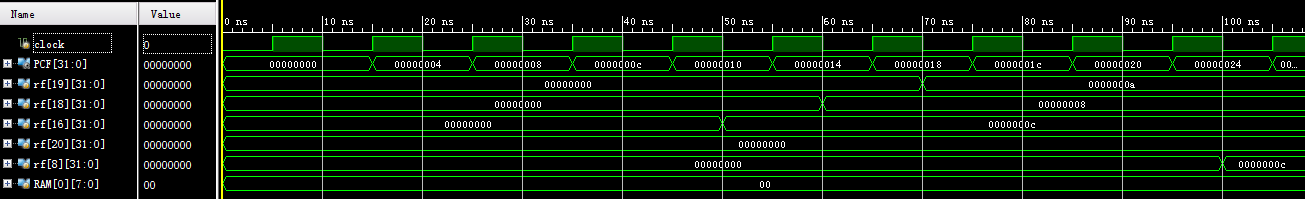
\includegraphics[width =\linewidth]{figure/all1.png}
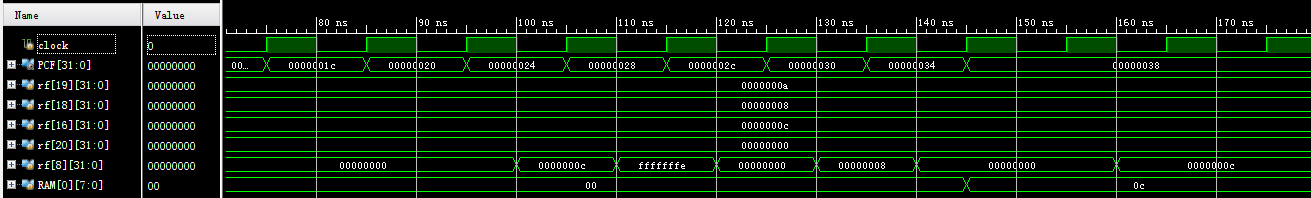
\includegraphics[width =\linewidth]{figure/all2.png}

上图中依次给出了寄存器 \$s3, \$s2, \$s0, \$s4 和 \$t0,以及内存地址0处的值。每条指令的结果依次应为:

\$s0 = 12 $\rightarrow$
\$s2 = 8 $\rightarrow$
\$s3 = 10 $\rightarrow$
\$s4 = 0 $\rightarrow$
nop $\rightarrow$
\$t0 = 12 $\rightarrow$
\$t0 = -2 $\rightarrow$
\$t0 = 0 $\rightarrow$
\$t0 = 8 $\rightarrow$
\$t0 = 0 $\rightarrow$
0(\$0) = 12 $\rightarrow$
\$t0 = 12


\subsection{gcd.in}

\begin{lstlisting}
 0x0 : addi $v0,$0,189      | 200200bd
 0x4 : addi $v1,$0,287      | 2003011f
 0x8 : main:                | 
 0x8 : beq $v0,$v1,end      | 10620007
 0xc : slt $at,$v0,$v1      | 0043082a
0x10 : beq $at,$0,run       | 10010003
0x14 : add $at,$v0,$0       | 00400820
0x18 : add $v0,$v1,$0       | 00601020
0x1c : add $v1,$at,$0       | 00201820
0x20 : run:                 | 
0x20 : sub $v0,$v0,$v1      | 00431022
0x24 : j main               | 08000002
0x28 : end:                 | 
0x28 : add $t3, $0, $0      | 00005820

\end{lstlisting}

这个测试样例是从黄文皓同学那里借来的,通过循环计算两个数的最大公约数。开始时,我们把需要计算的两个数字189和287分别赋值给\$v0和\$v1。之后,通过辗转相减法计算最大公约数。当\$v0与\$v1相等时,说明计算得到了它们的最大公约数。

\noindent
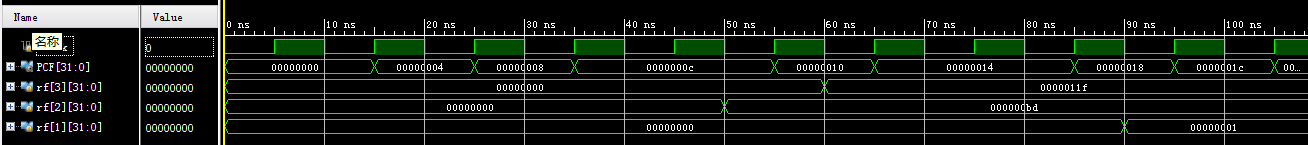
\includegraphics[width =\linewidth]{figure/gcd1.png}
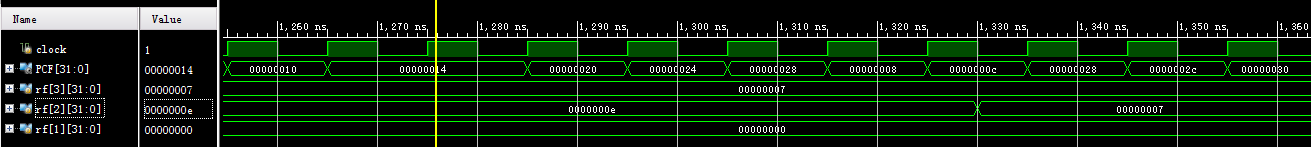
\includegraphics[width =\linewidth]{figure/gcd2.png}

这里的两幅图分别展示了程序开始与结束时的计算结果。从第一幅图可以看到程序正常的执行循环,后一幅图则说明程序成功地计算出两数的最大公约数为7。


\subsection{quick\_multiply.in}

\begin{lstlisting}
 0x0 : addi $t0, $0, 99     | 20080063
 0x4 : addi $t1, $0, 37     | 20090025
 0x8 : addi $s0, $0, 0      | 20100000
 0xc :                      | 
 0xc : while:               | 
 0xc : beq $t1, $0, done    | 10090006
0x10 : andi $t2, $t1, 1     | 312a0001
0x14 : beq $t2, $0, target  | 100a0001
0x18 : add $s0, $s0, $t0    | 02088020
0x1c : target:              | 
0x1c : sll $t0, $t0, 1      | 00084040
0x20 : srl $t1, $t1, 1      | 00094842
0x24 : j while              | 08000003
0x28 :                      | 
0x28 : done:                | 
0x28 : add $t3, $0, $0      | 00005820
\end{lstlisting} 

这个代码曾在单周期处理器中演示过,用于计算两数的乘积,方法类似快速幂。首先将99与37写入\$t0和\$t1寄存器,然后进入循环,每次根据\$t1的末位是否为1,来决定是否向\$s0进行累加,然后每次\$t0乘2,\$t1右移一位。最终,计算结果存在\$s0中,应为0xe4f。这个测试样例测试了跳转、移位等指令,测试结果如下:

\noindent
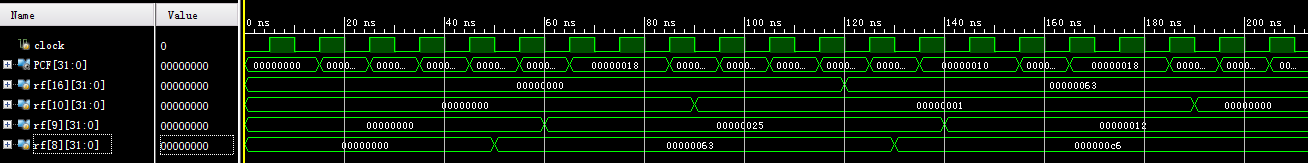
\includegraphics[width =\linewidth]{figure/mul1.png}
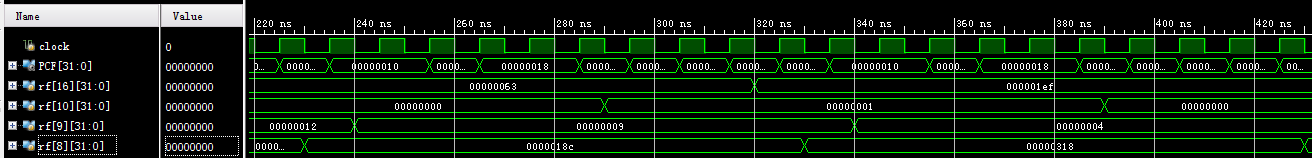
\includegraphics[width =\linewidth]{figure/mul2.png}
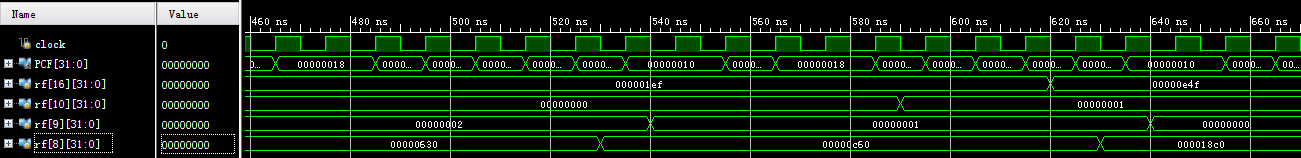
\includegraphics[width =\linewidth]{figure/mul3.png}

图中依次展示的是寄存器\$s0,\$t2,\$t1,\$t0的值,可以看到程序开始时,寄存器\$t0与\$t1分别被赋值为0x63与0x25,分别对应99与37。循环过程中,\$t0每次乘2,\$t1每次除以2,最终\$s0变为0xe4f,结果正确,说明程序正确执行。



\section{注意事项}

\subsection{遇到的问题}

想了一下,好像没啥问题。。。

\subsection{显示模块}

这次的显示模块和上次一模一样,不需要做任何改动。不过为了方便演示,我加入了一个暂停功能:

以sel信号作为调整时钟快慢的信号,以stop信号来控制是否暂停。当stop为1时,直接将0作为时钟信号传入即可。

\section{申A理由}

\begin{itemize}
\item 实现了所有的基本指令
\item 增加了移位指令sll,srl,sra
\item 增加了与函数调用相关的跳转指令jal,jr
\item 增加了乘法指令mul
\item 为乘法指令和函数调用指令添加了相应的测试样例
\end{itemize}

\end{sloppypar}
\end{document}
